\chapter{Soluzione Proposta}\label{chap:soluzioneproposta}

\section{Introduzione} \label{sec:solIntroduction}

L'estrazione dei dati dalla blockchain di Bitcoin ha richiesto un analisi preliminare della tecnologia ed in particolare sul modo in cui vengono serializzati i dati dal client; questa prima analisi ha permesso di osservare la rapida crescita dello spazio richiesto della blockchain, rappresentata dalla Figura \ref{fig:dimensionBlockchain}.

{\vspace{15pt}
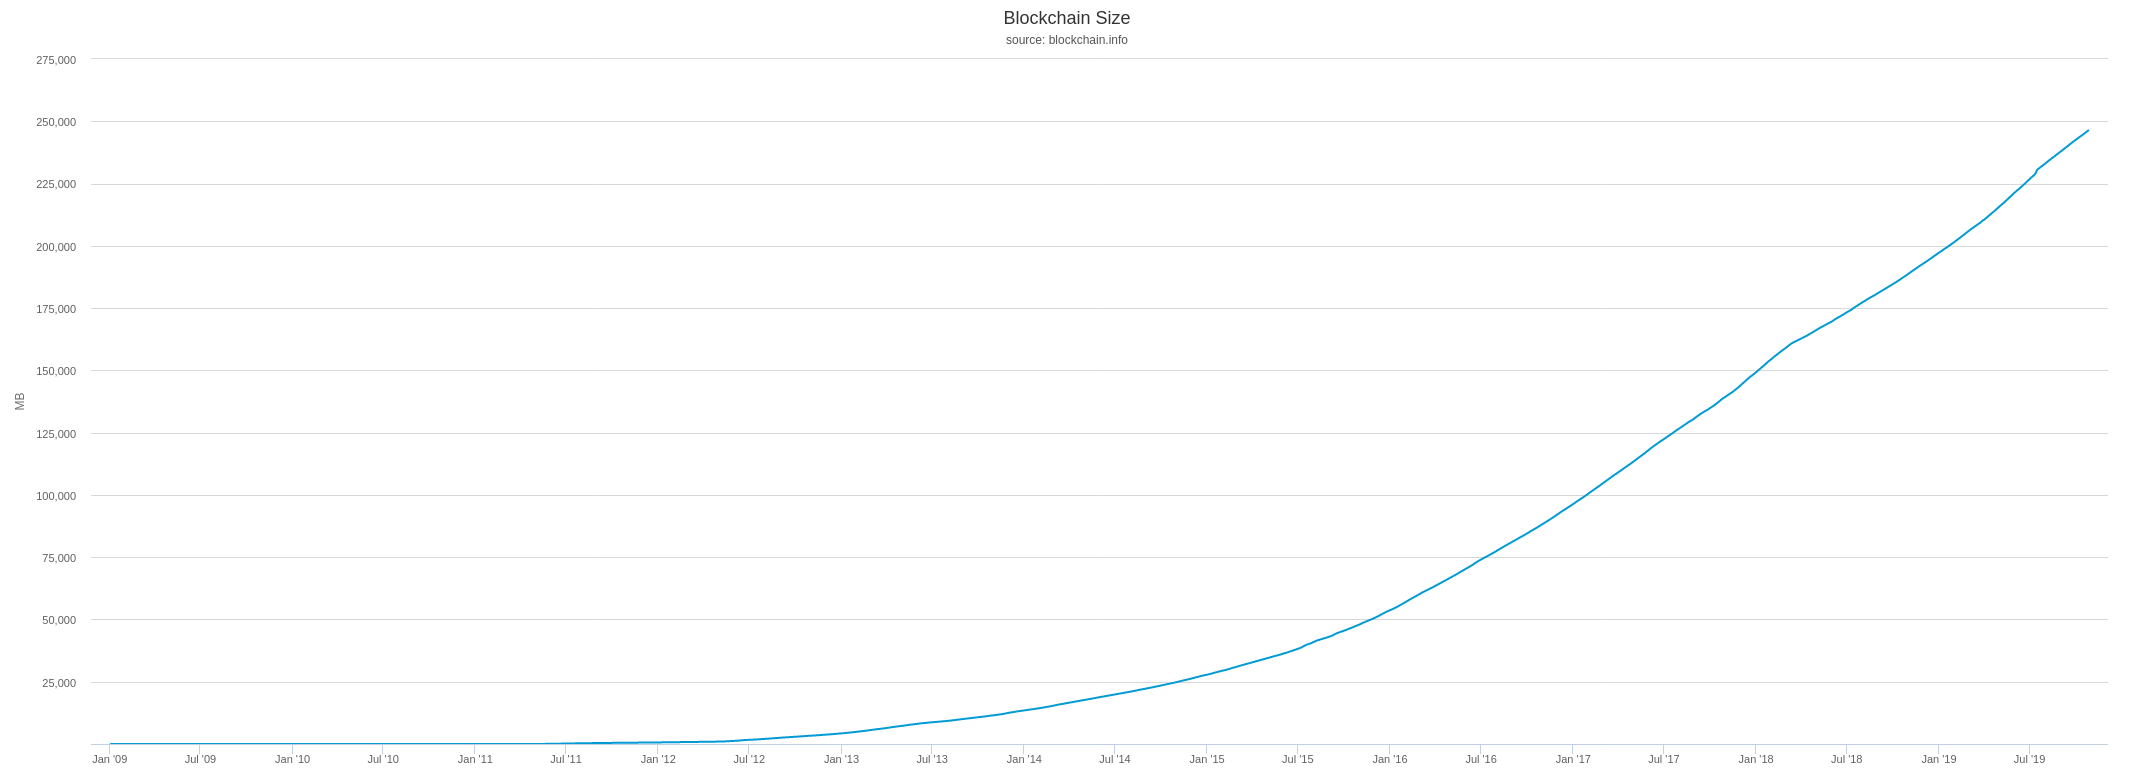
\includegraphics[scale=0.18]{images/blockchain-size.png}
\captionof{figure}{Rappresentazione della crescita della dimenzione della blockchain di Bitcoin nel tempo.\label{fig:dimensionBlockchain}}
\vspace{10pt}
\par}

La rapida crescita della blockchain porta alle seguenti problematiche:

\begin{itemize}
  \item L'estrazione dei dati dalla blockchain di Bitcoin richiede un software scalabile per permettere in qualsiasi condizione di utilizzo l'estrazione dei dati.
  \item L'organizzazione dei dati estratti della blockchain deve essere versatile per consentire analisi differenti; così da non costringere una seconda scansione a seconda del tipo di analisi da effettuare.
\end{itemize}

\section{SpyCBlock} \label{sec:spycblock}

SpyCBlock rappresenta la soluzione proposta per l'estrazione di dati dalla blockchain di Bitcoin in modo scalabile, con cui viene effettua la creazione dei due principali grafi per l'analisi forense, inoltre produce in formato JSON (JavaScript Object Notation) una deserializzazione completa delle blockchain con l'aggiunta di informazioni addizionali, infatti come descritto nel Capitolo \ref{chap:bitcoin} i blocchi e le transazioni contengono solo gli identificativi dei loro predecessori, costringendo il parser in fase di deserializzazione a ricostruire l'hash della transazione e del rispettivo blocco preso in analisi; questo è stato reso possibile dalla libreria descritta nel Capitolo \ref{sec:cryptographyBitcoinLib}.\\
SpyCBlock rappresenta un prototipo di un software di analisi accademico, sviluppato interamente in C++14, risiede su Github sotto licenza Apache License 2.0, esso è implementazione di un parser delle informazioni serializzate dal nodo Bitcoin; utilizzando le librerie descritte nella Sezione \ref{sec:bitcoinCoreLib}.\\
Il software è stato implementato utilizzando una metodologia Agile, infatti lo sviluppo di SpyCBlock e lo studio della tecnologia Bitcoin sono avvenute in parallelo, questo ha permesso di convalidare tutte le nozioni studiate sulla tecnologia, basando l'intero ciclo di sviluppo sulla produzione di test di unità (9 batterie di test, per un totale di 46 test di unità).\\
I dati decodificati del singolo blocco vengono verificati all'interno dei test di unità utilizzando dati prototti attraverso l'utilizzo di altri parser, tipo \cite{parser:blocktools} e attraverso i dati esposti dagli explorer, tipo \cite{blockstream:esplora} e \cite{blockchain:explorer}.\\

\section{Serializzazione della blockchain in formato JSON} \label{sec:spycblock}

Prima di effettuare la creazione dei grafi, descritti nelle sezioni successive, abbiamo dovuto affrontare varie problematiche incorse durante la fase di decodifica delle informazioni, infatti l'aggiornamento al Segregated Witness (descritto nella Sezione \ref{sec:transazionibitcoincore}) ha introdotto alcune modifice anche nel modo in cui viene serializzata una transazione; questo costringe il parser a utilizzare a seconda del tipo di transazione metodi diversi di deserializzazione.
L'aggiornamento al Segregated Witness ha introdutto tre nuove informazioni all'interno delle transazioni, che sono:
\begin{itemize}
  \item La proprietà flagh.
  \item La proprietà Marker.
  \item Se le due propietà precedenti sono rispettivamente 0 e 1 allora all'interno della transazione esisterà una lista di Script Witness, descritti nel Paragrafo \ref{sec:transazionibitcoincore} in cui vengono denominati \say{TransactionWitness}.
\end{itemize}

Il Frammento di codice descritto nella Sezione \ref{sec:decodeTransactionCode} rappresenta il codice con cui è possibile deserializzare una transazione dopo l'aggiornamento al Segregated Witness (viene usato Python per brevità).\\
I problemi relativi alla deserializzazione dei dati aggiunta all'enorme quantità di dati da deserializzare\footnote{ad oggi in data \today  l'attuale dimensione della blockchain di Bitcoin è pari a 270 Gb} ha richiesto la progettazione di un metodo di testing automatico sull'intera blockchain oppure su un parte specifica.
Questo ha richiesto di convertire le informazioni deserializzate dal parser in un formato file universale per eseguire il caricamento di queste informazioni con qualsiasi linguaggio.\\
Il formato file utilizzato per la codifica delle informazioni è il formato JSON (JavaScript Object Notation) e la libreria descritta nella Sezione \ref{sec:rapidjsonLib} ha reso possibile la serializzazione delle informazioni lette dal parser in maniera istantanea, cioè ogni blocco decodificato veniva serializzato in JSON istantaneamente con la conseguenza di un utilizzo di memoria RAM irrisorio.\\
L'adozione del formato JSON per l'organizzazione dei dati porta i seguenti benefici:
\begin{itemize}
  \item I dati serializzati in JSON possono essere testati in maniera automatizzata attraverso l'uso di API esterne oppure attraverso il framework RPC di Bitcoin-core descritto nella Sezione \ref{sec:jsonrpchttp}.
  \item I dati serializzati in JSON possono essere testati a vari livelli di precisone, ad esempio: Un eventuale errore di deserializzazione in un determinato punto della blockchain può essere individuato facilmente e osservato attraverso il suo rispettivo formato JSON.
  Questo evita l'uso del debugger per errori introdotti in fase di sviluppo dal programmatore e facilmente individuabile se i dati sono convertiti in un formato comprensibile per l'uomo.
  \item La rappresentazione JSON dell'intera blockchain offre anche la possibilità di eseguire ulteriori tipi di analisi all'interno della blockchain di Bitcoin, ad esempio attraverso l'utilizzo di una demo di analisi descritta nella Sezione \ref{sec:solDemo} è possibile utilizzare i dati in formato JSON per un analisi sui tipi di Script utilizzati all'interno della blockchain.
  In Figura \ref{fig:chartOPRETURN} viene riportato un grafico che rappresenta l'utilizzo estensivo dell'operatore OP\_RETURN (descritto nella Sezione \ref{sub:sectionNUllaDataScript}) e quindi l'utilizzo della blockchain di Bitcoin per l'archiviazione di dati.
\end{itemize}

{\centering
\vspace{15pt}
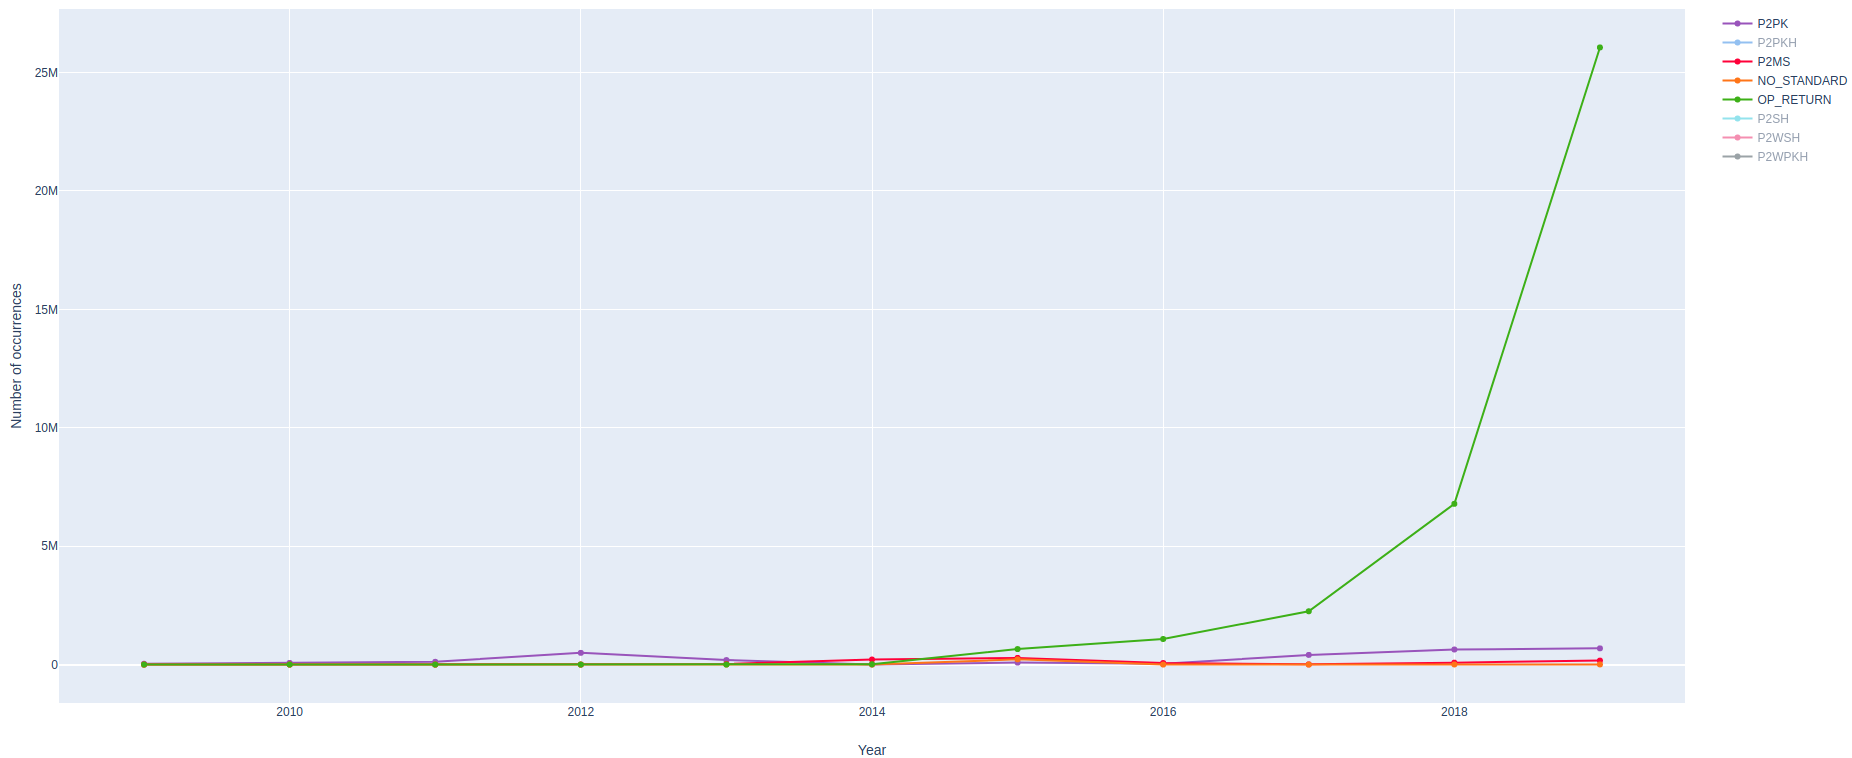
\includegraphics[scale=0.5]{images/OP_RETUTN_chart.png}
\captionof{figure}{Frammento di grafico estrapolato dalla demo \ref{sec:solDemo} dove viene rappresentato l'utilizzo del operatore OP\_RETURN all'interno degli script di blocco.\label{fig:chartOPRETURN}}
\vspace{10pt}
\par}


\section{Grafo delle transazioni} \label{sec:solGraphTX}

Dopo un accurata convalida dei dati deserializzati dal parser, abbiamo eseguito una nuova iterazione all'interno del ciclo di sviluppo del software, aggiungendo all'interno del parser la possibilità di serializzare i dati letti come arco di un grafo orientato.\\
Ogni transazione infatti genera un arco (u, v) in cui il nodo di origine (u) è rappresentato dall'hash della transazione attualmente analizzata e il nodo di arrivo (v) viene rappresentato dall'hash della transazione precedente, contenuta all'interno del tipo di dato \say{Outpoint} nella transazione di input (illustrato nella Sezione \ref{sec:transazionibitcoincore}).\\
Come descritto nella Sezione \ref{sec:grafoDelleTransazioniProblema} la creazione del grafo delle transazioni risulta abbastanza intuitiva, ma la strutture dati della blockchain di Bitcoin costringe il parser al calcolo dell'hash della transazione attualmente analizzata perchè esso non viene incluso; per fare questo il parser riconverte in memoria i dati nel formato di serializzazione originario.
In seguito alla riconversione con l'utilizzo della libreria \ref{sec:cryptographyBitcoinLib} viene eseguito il doppio SHA256 dei bit riguardanti le informazioni in formato esadecimale, in cui ogni tipo della struttura viene prima convertito nel formato little-endian.\\

\begin{example}

Prendiamo in considerazione la transazione coinbase del blocco di genesi\footnote{Il blocco di genesi è anche conosciuto come blocco 0 oppure blocco \emph{never mined}, i cui dati sono stati codificati da Satoshi Nakamoto all'interno del codice sorgente di Bitcoin-core. Introdurre dei nuovi dati all'interno del blocco di genesi implica la creazione di una nuova blockchain.} rappresentata nella Figura \ref{fig:txGenesisBlock}.

{\centering
\vspace{15pt}
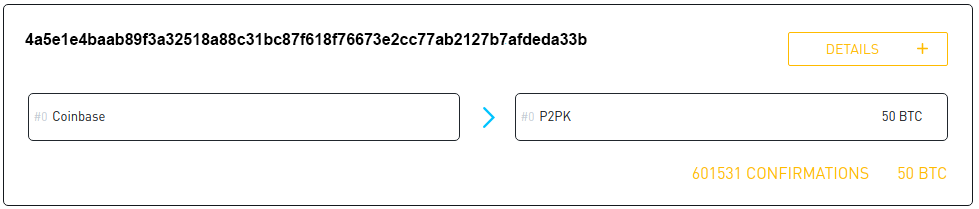
\includegraphics[scale=0.35]{images/coinbase_tx_genesis_block.png}
\captionof{figure}{Rappresentazione attraverso un'explorer \cite{blockstream:esplora} della transazione coinbase contenuta all'interno del blocco di genesi.\label{fig:txGenesisBlock}}
\vspace{10pt}
\par}

Analizzando i dati estratti dal parser possiamo notare che gli explorer non mostrano molte delle informazioni contenute all'interno delle transazioni, utilizzando il frammento di serializzazione JSON descritto nella Sezione \ref{sec:genesiBlockTxJSON} in cui viene raffigurata la prima transazione nella blockchain di Bitcoin, possiamo notare tutte le informazioni realemnte contenute nella struttara di una transazione.
Per effettuare il calcolo dell'hash della transazione il parser riconverte ogni tipo di dato nel formato little-endian e infine converte il valore nel corrispettivo esadecimale, la porzione di Codice C++ \ref{code:typehexTxCpp} riporta il valore convertito con il processo descritto in predecenza.

\lstinputlisting[language=C++, label=code:typehexTxCpp, caption=Frammento di codice C++ che rappresenta il valore esadecimale di ogni dipo di dato della transazione.]{code/coinBaseTxGenesisBlockHex.cpp}

Infine il codice \ref{code:processBuilHashTx} riporta un test di unità del progetto SpyCBlock in cui si effettua il processo di creazione dell'hash completo.


Dopo aver ottenuto l'identificativo della transazione il parser procede nella serializzazione della transazione come un arco (u, v) aggiungendo delle informazioni addizionali all'arco, tipo: l'altezza del blocco calcolato durante il parsing, quest'ultimo corrisponde alla sua posizione nella catena della blockchain.
Inserendo il valore calcolato come informazione dell'arco si evita di inserire l'hash del blocco in cui risiede la transazione, questo implica un notevole risparmio di spazio delle informazioni serializzate; inoltre vengono inseriti anche i valori corrispondendi al numero di bitcoin spediti e il valore nLockTime.\\
La serializzazione delle informazioni avviene in streaming, cioè ogni blocco letto viene immediatamente convertico nel file contenente tutte le informazioni delle transazioni, ottenendo un formato come quello rappresentato dal Codice \ref{code:archExampleTxGrapg}.\\

\lstinputlisting[label=code:archExampleTxGrapg, caption=Informazioni della transazione in Figura \ref{fig:txGenesisBlock} decodificata nel'arco corrispondente.]{code/exampleArch.txt}

\end{example}

Attraverso la serializzazione delle transazioni con formato appena descritto è possibile facilmente realizzare un applicativo web per la visualizzazione del grafo utilizzando la libreria javascript descritta nella Sezione \ref{}; ottenendo cosi una porzione di grafo descritta dalla Figura \ref{fig:visgraphTx}, in cui si può notare l'enorme quantità di transazioni conentute in una piccola parte di blockchain (50 Mb di 270 Gb) che rende difficile il rendering di esse.
Attraverso alcuni zoom effettuati si può notare l'esistenza di piccole comunità di nodi che scambiano bitcoin; in particolare possiamo notare dallo zoom \say{B} dei nodi che fanno parte di transazioni M:1.
\newpage
{\centering
\vspace{15pt}
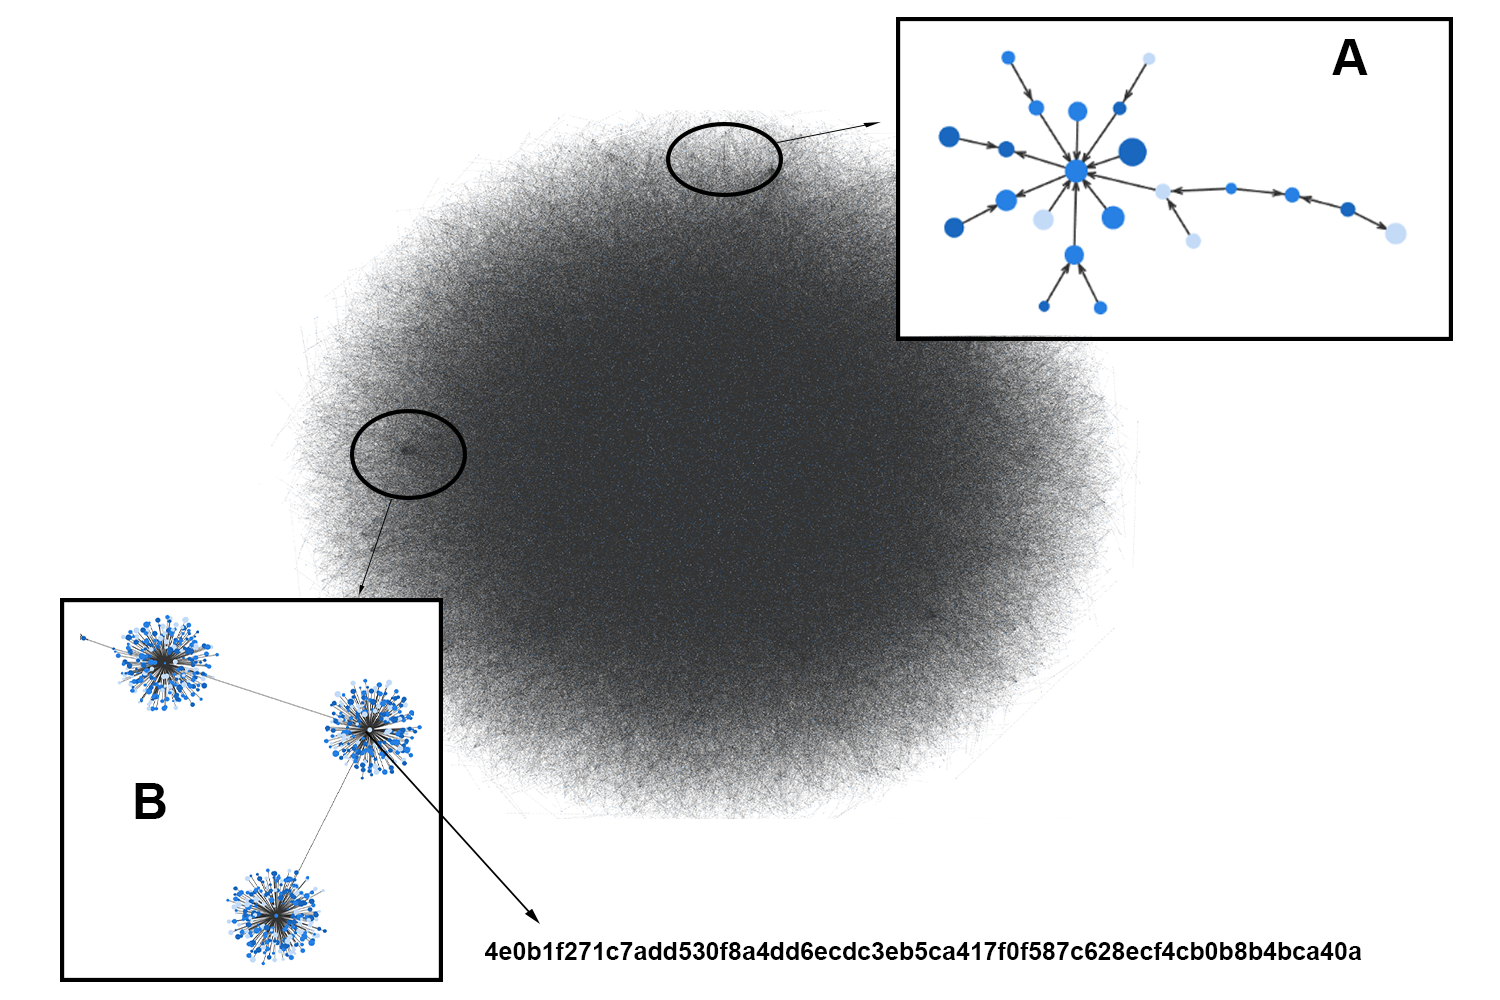
\includegraphics[width=80mm, scale=0.5]{images/demo/graph_tx_demo_presentation.png}
\captionof{figure}{Rappresentazione di una porzione di grafo delle transazioni attraverso la demo descritta nella Sezione \ref{sec:solDemo}.\label{fig:visgraphTx}}
\vspace{10pt}
\par}

\begin{example}
  Prendendo in esempio lo zoom \say{B} della Figura \ref{fig:visgraphTx} possiamo notare 3 comunità di nodi, in cui solo uno di esso spedice bitcoin ad un altra comunità.\\
  Prendendo in considerazione il nodo con il segunte identificativo di transazione \say{4e0b1f\-271c7add\-530f8a4dd6e\-cdc3eb5ca41\-7f0f587c6\-28ecf4cb0\-b8b4b\-ca40a}, si può notare attraverso l'uso di uno explore che la transazione contine 236 transazioni di input e 1 transazione di output, questo potrebbe significare che il wallet abbia raggruppato tutte le transazioni su un unico address.
\end{example}

Inoltre la blockchain di bitcoin serializza i blocchi all'interno di file chiamati \say{blk00000.dat} dove \say{00000} rappresenta l'indice dei file; Bitcoin-core stabilisce degli standard di dimensione per i file, pari a 100 Mb per ogni file.\\
SpyCBlock effettua la serializazione 1 a 1, cioè per ogni file \say{blk0000.dat} produce un file con le informazioni in un specifico formato ad esempio \say{blk00000.json}, questo da la possibilità di far evolvere facilmente il parser ad un implementazione multiprocessore.

\section{Grafo degli address} \label{sec:solGraphAddress}

In seguito alla costruzione del grafo delle transazioni, ci siamo concentrati sulla costruzione del grafo degli address, come descritto nella Sezione \ref{sec:grafoDegliAddressProblema} la costruzione del grafo introduce ad alcune problematiche che costringono a rivedere il modo in cui si ricavano i dati durante il parsing delle informazioni.\\
Infatti gli address sono contenuti solo all'interno dello script di blocco di una transazione e come illustrato nelle Sezioni \ref{sec:bitcoinScriptBitcoin} e \ref{sec:bitcoinScriptBitcoinCore} lo script di sblocco contiene informazioni riguardanti le condizioni per cui un UTXO può essere sbloccato e quindi esso non possiede nessun riferimento all'indirizzo di origine.
Per accedere allo script di blocco della precedente transazione, il cui identificativo (hash) risiede all'interno della transazione di input appartenente alla transazione attualmente analizzata bisogna memorizzare la cronologia delle transazioni decodificate e ricostruire un meccanismo per la gestione degl'UTXO, simile al meccanismo usato da Bitcoin-core: cioè adibire un metodo di memorizzazione che consente di prelevare una transazione precedentemente analizzata con costo O(1) oppure con un costo lineare O(N).\\
Inoltre al momento della stesura del documento il parser non possiede nessun meccanismo di analisi degli script; perchè essi con il passare del tempo sono diventati molto complessi, e come visto nella Sezione \ref{sec:noStrandardScript} vengono introdotti metalinguaggi (tipo miniscript) per la facilitare la scrittura di \say{script no standard}; questo introduce ad una problematica che porta alla necessità di studiare in modo accurato gli script per ricavare attraverso l'analisi di essi maggiori informazioni che consentono di effettuare una catalogazione più accurata.
 \begin{example}\label{ex:probleGraphAddress}
   Prendendo in considerazione l'address \say{3CD1\-QW6fjg\-TwKq3Pj\-97nty28W\-ZAVkz\-iNom} coinvolto in numerose truffe e illustrato all'interno dell'articolo \cite{biva:article} dove possiamo notare che l'address è originato da uno script, perchè esso utilizza la convenzione del numero 3 come prima cifra; quest'ultimo potrebbe contenere più address primitivi al suo interno e quindi rappresentare uno script P2MS oppure potrebbe rappresentare un'address ricavato da uno script no standard, un esempio di script no standard è illustrato attraverso il Codice \ref{code:complexscript}.\\
   Gli address originati da script costringono ad un analisi più approfondita per ricavare maggiori informazioni sulla loro vera identità; come illustrato nella Sezione \ref{sec:p2shBitcoin} lo script P2SH è il primo esempio di script ad introdurre la possibilità di generare un'address non primitivo, in seguito si aggingono anche P2WSH, P2WPKH e gli script no standard.\\
   Inoltre possiamo osservare dalla Sezione \ref{sec:p2shBitcoin} il processo di verifica per uno script P2SH; dove per sbloccare un UTXO bloccato attraverso uno script P2SH bisogna fornire oltre alle firme delle chiavi private anche lo script P2MS (reedmeScript) da cui è stato originato l'hash inserito all'interno dello script di blocco; questo costringe ad analizzare oltre lo script di blocco anche lo script di sblocco.\\
   Considerando la transazione con identificativo \say{82\-a69\-be69e\-00937\-91ab7\-d3803\-69ec\-ffba4f\-1fe08\-27a862\-5ede9\-d89e9\-4776b\-c21} bloccata attraverso lo script da cui è originato l'address \say{3CD1\-QW6fjg\-TwKq3Pj\-97nty28W\-ZAVkz\-iNom} possiamo osservare che essa viene \say{consumata} dalla transazione con il seguente identificativo \say{457\-b5bde2\-35dcf08\-de41597\-68c4f7\-abcb96\-97e1\-760a\-13e6\-caa15a\-7a2d8\-c909\-78}, quest'ultima all'interno dello script di sblocco contiene le informazioni necessarie per lo sblocco della transazione bloccata dall'address \say{3CD1\-QW6fjg\-TwKq3Pj\-97nty28W\-ZAVkz\-iNom}.
   Lo script di blocco da cui è originato l'address viene illustrato attraverso il Codice \ref{code:scriptPubKeyScam} dove possiamo osservare che il corrispettivo script appartiene alla cerchia di script standard ed in particolare è uno script P2MS.
   \begin{lstlisting}[language=bitcoinscript, label={code:scriptPubKeyScam}, caption={Script da cui è originato l'address preso in esempio.}]
      OP_HASH160 735d4de855597997b21588cc78ca2db696be1c5d OP_EQUAL
   \end{lstlisting}
   Lo script capace di sbloccare la transazione bloccata con lo script precedente è contenuta all'interno della transazione con il seguente identificativo \say{457\-b5bde2\-35dcf08\-de41597\-68c4f7\-abcb96\-97e1\-760a\-13e6\-caa15a\-7a2d8\-c909\-78}; il Codice \ref{code:scritpSigScam} illustra lo script di sblocco.
     \begin{lstlisting}[language=bitcoinscript, label={code:scritpSigScam}, caption={Script con cui è possibile eseguire con successo lo script illustrato attraverso il Codice \ref{code:scriptPubKeyScam}.}]
      OP_0 304402203638fc4c33f325d1c62c8feb4979d91300723f4766686e89de7380b269eec
        c7602206d65886d69ccedc33de8f2840f27295b53dd9f9fd637b970664385b47c128da901
        3045022100e8910b2162c08ec560d5737d09d361c07f90bfe58ee4e66a4fbebe246ea2b32c
        02207fb1fc6296213b11ecb2eef3a375c8509776f75880ad5372417b55215fcdf74f01
      OP_PUSHDATA1 522103385adff37fd3d0a620ebc4e9866e81dda8ba8616e5ebcae899c7f51899267
        ae721034c08511718f947d1a3e152195c5e2756588e3e0c2c7730927eb6647af494210721033d
        a9f8938a5b947a723df21b73fbd3985b719249324d2c705acfb97d63a5df9e53ae
     \end{lstlisting}
     Da cui possiamo estrarre lo script di ricatto contenuto dopo l'operatore OP\_PUSHDATA1, illustrato nel Codice \ref{code:p2msScam}.
     \begin{lstlisting}[language=bitcoinscript, label={code:p2msScam}, caption={Readme Script contenuto all'interno dello script di sblocco \ref{code:scritpSigScam}.}]
      OP_2 03385adff37fd3d0a620ebc4e9866e81dda8ba8616e5ebcae899c7f51899267ae7 034c08511718f947d1a3e152195c5e2756588e3e0c2c7730927eb6647af4942107 033da9f8938a5b947a723df21b73fbd3985b719249324d2c705acfb97d63a5df9e OP_3 OP_CHECKMULTISIG
    \end{lstlisting}
    Dal Codice \ref{code:p2msScam} si possono notare 3 chiavi pubbliche differenti:
    \begin{itemize}
      \item \say{0338\-5adff37\-fd3d0a62\-0ebc4e98\-66e81dd\-a8ba8616\-e5ebcae89\-9c7f518\-9926\-7ae7}.
      \item \say{034c\-0851\-1718f947\-d1a3e152\-195c5e2756\-588e3e0c2c\-7730927\-eb6647a\-f494\-2107}.
      \item \say{033\-da9f8\-938a5b9\-47a723df\-21b73fbd3\-985b719249\-324d2c70\-5acfb97d\-63a5\-df9e}.
    \end{itemize}
    Queste chiavi pubbliche rappresentato identità differenti appartenenti allo stesso wallet oppure a wallet differenti, utilizzando il codice descritto nella Sezione \ref{sec:buildAddressFromPubKey} possiamo ricavare un address primitivo dalle chiavi pubbliche, ottenendo i seguenti address.
    \begin{itemize}
      \item \say{14r7XjPtqVijLRhY9BkGAtDqVDp4txsK1X}.
      \item \say{1GryVw5pfa8a1Sc69PXywGLRDZJWc1C6wT}.
      \item \say{1G9VBMkqDzPmYxnFMkNxWGmfuQz1CHSYP6}.
    \end{itemize}

    Questo esempio illustra la necessità di analizzare approfontitamente gli address originati da script perchè essi sono sempre più diffusi all'interno della blockchain di Bitcoin e con essi si ottiene un maggiore livello di privacy.
    La creazione del grafo di address deve poter rappresentare il reale flusso di bitcoin tra address; ad esempio nel esempio appena descritto dove l'address  \say{3CD1\-QW6fjg\-TwKq3Pj\-97nty28W\-ZAVkz\-iNom} viene catalogato come address convolto in truffe ma analizzando attendamente lo script da cui è originato l'address si riesce a osservare che gli address coinvolti nella truffa sono 3.
    Non effettuando quest'ultima analisi, ogni singolo address potrebbe operare singolarmente all'interno della blockchain di Bitcoin passando inosservato agli algoritmi di analisi.
 \end{example}

 Attraverso l'Esempio \ref{ex:probleGraphAddress} possiamo notare due tipi di grafi di address che si possono costruire utilizzando le informazioni estratte dalla blockchain di Bitcoin, cioè:
 \begin{itemize}
   \item Il grafo naturale di address, utilizzando solo le informazioni contenute all'interno delgli script di blocco, ad esempio il frammento di grafo descritto dalla transazione illustrata nell'esempio \ref{ex:probleGraphAddress} con il seguente identificativo \say{82\-a69\-be69e\-00937\-91ab7\-d3803\-69ec\-ffba4f\-1fe08\-27a862\-5ede9\-d89e9\-4776b\-c21} rappresentato dalla Figura \ref{fig:addGrapjNatural}
   \begin{figure}[H]
   \centering
   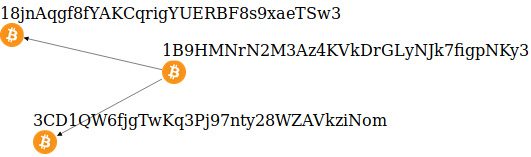
\includegraphics[scale=0.35]{images/exampleWithGraph/naturalAddressGrahScamTx.png}
   \caption{Frammento del grafo naturale degli address descritto dalla transazione con identificativo 82\-a69\-be69e\-00937\-91ab7\-d3803\-69ec\-ffba4f\-1fe08\-27a862\-5ede9\-d89e9\-4776b\-c21.\label{fig:addGrapjNatural}}
   \end{figure}
   Il grafo risulta essere una soluzione superficiale, perchè le chiavi pubbliche che fanno parte dello script da cui è ottenuto l'address \say{3CD1\-QW6fjg\-TwKq3Pj\-97nty28W\-ZAVkz\-iNom} potrebbero essere riutilizzate singolarmente all'interno della blockchain di Bitcoin passando inosservate agli algoritmi di analisi.
   \item Il grafo degli address ottenuto con un analisi degl'indirizzi originati da script, un esempio tratto dalla porzione di grafo illustrato nella Figura \ref{fig:addGrapjNatural} in cui è stata condotta un analisi sullo script \say{3CD1\-QW6fjg\-TwKq3Pj\-97nty28W\-ZAVkz\-iNom} è illustrato nella Figura \ref{fig:addGraphAnalisis}
   \begin{figure}[H]
   \centering
   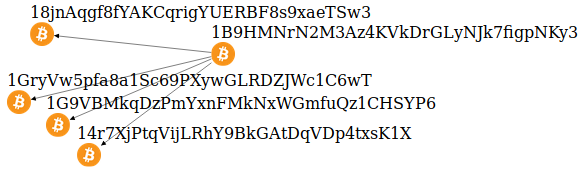
\includegraphics[scale=0.35]{images/exampleWithGraph/decode-address-graph-scam.png}
   \caption{Frammento del grafo degli address ottenuto attraverso un analisi dell'address 3CD1\-QW6fjg\-TwKq3Pj\-97nty28W\-ZAVkz\-iNom.\label{fig:addGraphAnalisis}}
   \end{figure}
 \end{itemize}


\section{DEMO} \label{sec:solDemo}
